\documentclass[12pt,a4paper,oneside]{book}

\usepackage[top=3cm, bottom=2cm, left=2cm, right=2cm]{geometry}
\usepackage[utf8]{inputenc}  % codificação dos caracteres acentuados
%\usepackage[T1]{fontenc}       % codificação da fonte (para hifenizar palavras com acentos)
%\usepackage[portuges]{babel}   % package para a hifenização e labels em pt
\usepackage{url}               % package para formatar urls
\usepackage[pdftex]{hyperref}  % package para criar urls no pdf
\usepackage{multirow}          % package para juntar linhas em tabelas
\usepackage{graphicx}          % package para inclusão de imagens
\usepackage{bigstrut}          % package para espaçamento usado pelo multirow
\usepackage{fancyhdr}          % package para alterar os header
\usepackage{fancyvrb}         % package para mais estilos de verbatim
\usepackage{listings}
\usepackage{pdfpages}
\usepackage{nameref}
\usepackage{makeidx}
%urlbst - sacar este style para bibliografia com urls

% include figure macro
% example:
% \fig{img/uno-card-game.jpg}{Uno Cards}{uno_cards}{0.5}
\usepackage{ifthen} 
\newcommand{\fig}[4]{
\begin{figure}[h]
	\begin{center}
    \includegraphics[scale=#4]{#1}
    \end{center}
	\ifthenelse{\isundefined{#2}}{}{\caption{#2}}
	\ifthenelse{\isundefined{#3}}{}{\label{#3}}
\end{figure}
}


\lstset{numbers=left,breaklines=true}
\lstset{language=perl,frame=ltrb,framesep=5pt, basicstyle=\small, 
keywordstyle=\ttfamily\color{blue}, 
commentstyle=\color{Green}, 
stringstyle=\ttfamily, showstringspaces=false}

\setcounter{tocdepth}{4}
\setcounter{secnumdepth}{3}
\makeindex

\begin{document}
\includepdfset{pages=-}

% COVER
\pagestyle{plain}
\begin{titlepage}      
	\begin{center}
		
\includegraphics{img/logoisep2.png}\\
	\end{center}
	
	\vfill
	\begin{center}
		\bf \LARGE Erasmusline: \\Executive Information System\\
		\ \\ \normalsize 2010 / 2011
	\end{center}
	
	\vfill
	\begin{center}
		\bf 1050053 Daniel Lopes\\
		1070462 Pedro Ferreira\\
	\end{center}
	
	\vfill
	\begin{center}
		
\includegraphics{img/logoisep.png}\\
	\end{center}
	

\end{titlepage}
%%%%%%%%%%%%%%%%%%%%%%%%%%%%%%%%%%%%%%
% contra capa
\newpage

	\vfill
	\begin{center}
		\bf \LARGE Erasmusline: \\Executive Information System\\
		\ \\ \normalsize 2010 / 2011
	\end{center}

	\vfill
	\begin{center}
		\bf 1050053 Daniel Lopes\\
		1070462 Pedro Ferreira\\
	\end{center}
	
	\vfill
	\begin{center}
		
\includegraphics{img/logoisep2.png}\\
	\end{center}
	
	\vfill
	\begin{center}
		\bf \Large Licenciatura em Engenharia Informática\\
		\ \\ \normalsize September 2011
	\end{center}
	
	\vfill
	\begin{center}
		ISEP Supervisor: \bf Prof. Nuno Escudeiro
	\end{center}
	
\newpage
\vfill
\begin{flushright}
	\begin{tabular}{|l| p{200px} |}
	\hline
	Score & ~\\
	\hline
	Observations & ~\\
	~ & ~ \\
	~ & ~ \\
	~ & ~ \\
	\hline
	Additional Info. & ~\\
	~ & ~ \\
	~ & ~ \\
	~ & ~ \\
	\hline
	\end{tabular}
\end{flushright}
\frontmatter

\pagestyle{fancy}

\titlepage\ \endtitlepage

\chapter*{Acknowledgments}


\chapter*{Abstract}
MUTW stands for Multinational Undergraduate Team Work. The
goal of MUTW is to let students of eleven different universities work together on one common project. The assignment of this year was to implement the ErasmusLine web application. The purpose of this application was to digitalize the complete Erasmus process, so that students who want to go on Erasmus didn’t have to fill in all the forms by hand, butt everything would happen digitally.


The eleven universities taken part in this project were separated into
two teams, namely team Orange and team Blue. Those two teams would then work for about three months on implementing the application and at the end of those three months, they would have to give a presentation with their final result.


The implementation of the application itself was divided in eight
modules, which were distributed among the universities in each team. By dividing this project in different modules, each university could work independently on their own module, but this made the communication part of the project very important. Although each university could work independently on their modules, nevertheless did some modules depend on others.


The web application was written in XHTML with PHP as server-side
scripting language. Besides XHMTL and PHP, the Orange Team also used the MySQL
database as a data layer and JavaScript/jQuery as client-side scripting
language. The course-matching module used the Python programming language. 

 
This assignment was a very enriching experience for the whole team.
During the implementation of the ErasmusLine web application, some issues were
encountered and bugs to fix, but eventually a working application was presented
at the final meeting in Heraklion, Greece.

\section*{Keywords}
Database, data-management, user-management, sql, security-levels, homepage,
main- menu, privileges, permissions, interoperability, interface, data transfer,
file transfer, encryption, security, JSON, 3DES, cURL, Erasmus, forms,
server-side, validation, client-side, persistence, process
flow, signatures, exams, interface, institution, coordinator, student,
statistics, analytics, trends, charts, pivot tables, data warehouse,data
refreshment, executive information system, EIS, online analytical processing,
OLAP, extract transform load, ETL, data mining, facts, dimensions, measures,
posix, daemon, mysql, php, html, jquery.
 %include keywords

% indices
\tableofcontents
\listoffigures
\listoftables

\chapter*{Glossary}

\mainmatter

\chapter{Introduction} \label{ch:intro}

\section{Project Scope} \label{sec:pscope}
The MUTW (Multinational Undergraduate Team Work) Project is created by teachers
and students from all over the Europe. It's main purpose is to collaboratively
design a functional web application which is going to help the undergraduate
students and coordinators avoid the bureaucracy of filling all the necessary
forms and speed up the process, in case they want to use the Erasmus Program,
and also keep statistical records of what is happening during each student's
Erasmus mobility process.

The site which is called \emph{Erasmusline} is approachable by the students by
using their unique password given by their University and of course by the
coordinators who will work as administrators for the site. Furthermore, this
project has deeper goals to be achieved. Students have to work all together for
three months in order to make the site completely functional. This requires
teamwork and communication spirit. As a result, the participants will not only
practice their English language skills, but also their skills in planning,
analysis and technical expertise.

\section{Project Description}

The participants are students from eleven different Universities throughout
Europe which use the Erasmus Program. Each University offers two students for
the project. Every university has its own unique part in the project to
prepare, and during these three months, pieces are getting together in order to
make the final result, the site.

Eventually, this project turns out to be a unique and valuable experience which
can open new doors to the team's academic world. The objective of the project 
is to create a totally functional website which is going to be used by all
actors involved in the Erasmus program, that includes the students and
coordinators.

The students will be able to fill the forms needed for getting accepted by the
University abroad and the coordinators will be able to log in as administrators,
so they will be having access in every form in order to make the appropriate
moves for communicating with the other University.

Coordinators and students will also be able to consult global and institutional
statistics, generally for decision making - for example, students who seek to
study in institutions with specific traits - and detecting trends or anomalies
- in case of executive staff members who need to analyze the Erasmus process
success or failure in their own institution.

The beginning of the project took place in Kiel,Germany where all the
participants met for the first time and each team made its first view of the
project in a presentation. That presentation included the theoretical timeline
until the final presentation and what was the plan for creating the website step
by step.

There are two teams which take part in the project, the Orange and Blue
teams. Each team consists of six Universities from all over Europe and in the
final presentation the coordinators will evaluate each team according to the
work which was done these three months and the presentation itself.
Participants are gonna be also evaluated separately one by one.

This Project report will account for the process of planning and development of
the Orange team, but mainly for the Portuguese members and their assigned
project package, P8-STATS.

\subsection{Project Planning}

The Project development was controlled using the software tool
OpenProj\footnote{http://openproj.org} and editing the existing Gantt Chart,
accessible by the team's members in the SourceForge Git
repository\footnote{http://mutworange.git.sourceforge.net/}.

Every package member was responsible for filling out
their package Work Breakdown Structure, assign each deliverable time boxes and
regularly filling the percentage of their work done.

\fig{img/gantt_openproj.png}{The project's Gantt Diagram on
OpenProj}{img:gantt_openproj}{0.6}

The detailed Gantt Chart can be found in the chapter \emph{\nameref{apx5}}, page
\pageref{apx5} of this report.


Apart from checking the project's and each individual package's performance, the
team acted on democratic decision - when selecting the tools, when resolving
open ended questions – recurring to presential meetings through the software
tool Adobe Connect\footnote{http://www.adobe.com/products/adobeconnect.html},
IRC channels, direct email and the SourceForge Mailing List system.


Given the democratic nature of the team, each package team would also
self-manage their own package planning, using their own tools but always
reporting to a general Gantt Chart.

\ \newline
This project was developed during the second semester of 2011, between the
21$^{st}$ of March and the 17$^{th}$ of June. The following description lists
show each packages main tasks and milestones, each with their corresponding
time box - according to each country member's perspective.

\ \newline
\textbf{P1-CONFIG (Germany)} 
\begin{itemize}
\item Database \hfill 21/03 – 29/04 \begin{itemize}
  \item Design
  \item SQL Script
  \item Installation Script
\end{itemize}
\item Design \hfill 25/03 – 15/04 \begin{itemize}
  \item Design Mock Templates
  \item Integration with Plonk Templating library
\end{itemize}
\item User Account \hfill 18/04 – 29/04 \begin{itemize}
  \item Login functionality
  \item User roles and permissions
  \item Account page
\end{itemize}
\end{itemize}

\ \newline
\textbf{P2-INFOX (Germany)} 
\begin{itemize}
\item Discussion about communication Protocol \hfill 28/03 – 01/04
\item Define Security System \hfill 04/04 – 29/04
\item Programming Outgoing data	\hfill 02/05 – 13/05
\item Programming Incoming data	\hfill 02/05 – 13/05
\end{itemize}


\ \newline
\textbf{P3-ALERT (Bulgaria)} 
\begin{itemize}
\item Research	\hfill 22/03 – 06/04
\item Making the daemon	 \hfill 07/04 – 20/04
\item Synchronization with the others part of the project	\hfill 21/04 – 27/04
\item Email sending system	\hfill 28/04 – 05/04
\item Pop-ups	\hfill 28/04 – 05/04
\item GUI		\hfill 05/05 – 09/05
\item Testing	\hfill 10/05 – 23/05
\end{itemize}


\ \newline
\textbf{P4-OUT (Belgium)} 
\begin{itemize}
\item Collect Different forms	\hfill14/03 – 01/04
\item Setting up chart with the form flow	\hfill25/03 – 29/03
\item Agree with P-IN on layout forms		\hfill28/03 – 01/04
\item Determine which forms can be common		\hfill04/04 – 08/04
\item Implement non/common forms		\hfill11/04 – 29/04
\item Creating ECTS forms		\hfill28/03 – 01/04
\item Implement flow of forms		\hfill11/04 – 10/05
\item Integrate information  exchange module		\hfill18/04 – 22/04
\item Intensive testing of flow		\hfill10/05 – 31/05
\end{itemize}


\ \newline
\textbf{P5-IN (Greece)} 
\begin{itemize}
\item Research 
\item Develop the IN student forms
\item Testing
\item Report
\end{itemize}

\ \newline
\textbf{P6-EXAM (Bulgaria)} 
\begin{itemize}
\item Research
\item Making the student module
\item Making the home coordinator module
\item Making the host coordinator module
\item Synchronization with other parts of the project
\item Testing
\item Report
\end{itemize}

\ \newline
\textbf{P7-MATCH (Iceland)} 
\begin{itemize}
\item Research
\item Develop data scrapper to match dummy data
\item Develop production code
\item Integration tests
\item Testing
\item Report
\end{itemize}

\subsection{Project Meetings}

\section{Project Contributions}

\section{Report Structure}

\chapter{Context} \label{ch:context}

\section{Specifications} \label{sec:specs}

The MUTW Erasmus site – called ErasmusLine – is a web application
providing a platform to support Erasmus mobility of students.

All actors involved in Erasmus mobility, including students, Erasmus
coordinators, International Office and other staff, are granted access to the
platform. The ErasmusLine platform must provide ways to manage all the Erasmus
activity of the institution related to students’ mobility. Supporting the
bureaucratic process accompanying students’ mobility from the application stage
until the academic recognition includes several tasks, such as:

\begin{itemize}
  \item Inter-institution process documentation exchange
  \item Take exams at host institution
  \item Issue automatic alerts for required actions
  \item Match learning agreement to students’ requirements, with an automatic
  course matching facility
\end{itemize}

Additionally we want to evaluate the performance of institutions and students in
operating these procedures and Erasmus dynamics in each institution. This
involves some extra functionality:

\begin{itemize}
  \item Produce performance statistics
  \item Provide tools to analyze these statistics.
\end{itemize}

The ErasmusLine system is composed by four core areas: \emph{business,
statistics, services} and \emph{configuration}, as depicted in Figure
\ref{img:cores}. \newline

\fig{img/cores.png}{ErasmusLine Core Areas}{img:cores}{0.7}

The business core is responsible for the workflow of Erasmus exchanges, both for
outgoing and incoming students. It includes four packages directly related to
managing the Erasmus processes: “OUT students”, “IN students”, “Exams at host
institution” and “Course Matching”.

The services core provides a set of services available throughout the
ErasmusLine system. These services are deployed by the packages “Information
exchange and security” and “Automatic alerts”.

The configuration core is responsible for assuring that all the required data is
available and coherent. This core is implemented by the “Configuration” package.

The statistical core - developed by the Portuguese team - is an Executive
Information System (EIS) designed to provide statistical information to analyze
the performance of institutions and the interest of students regarding Erasmus
mobility.

These Core Areas include 8 distinct packages, depicted in Figure
\ref{img:packages}:

\fig{img/packages.png}{ErasmusLine Package Distribution}{img:packages}{0.7}

\begin{description}

\item[P1-CONFIG]
This package is responsible for parameter and entity management. All other
packages will rely on this one to get validated, coherent data required to
operate the system. User accounts and user profiles are also managed by this
package.

\item[P2-INFOX]
This package allows exchanging documents and students’ processes between
instances of the ErasmusLine application.

\item[P3-ALERT]
This package generates automatic alerts for pending tasks. These alerts are
triggered by timeouts associated to requests that are not answered in due time.

\item[P4-OUT]
This package assists \textbf{outgoing} students, home coordinators and staff in
the management of the exchange process from pre-candidacy to the conversion of the
ECTS credit to a local scale.

\item[P5-IN]
This package assists \textbf{incoming} students, host coordinators and staff in
the management of the exchange process from application submission to the
issuing the transcript of records.

\item[P6-EXAM]
Whenever Erasmus students have mandatory courses, for which there are no
interchange options in the host institution, they can request to take the exam
on that course at the host institution.

\item[P7-MATCH]
This package will perform an automatic matching of courses based on textual
descriptions offered by the host institution and the student’s needs.

\item[P8-STATS]
This package deploys an Executive Information System that collects operational
data and exposes it to users through a set of statistical indicators designed to
provide ways to evaluate the performance of these processes, to identify
critical tasks and to evaluate the Erasmus impact and progress in the
institutions.

\end{description}

\section{P8-STATS Erasmus Statistics}
This statistics module – an Executive Information System (EIS) – is responsible
for collecting operational data from ErasmusLine databases and, eventually, from
some external sources, in order to compute performance statistics that comply
with the objectives to be controlled. It should also provide an interface that
exposes these indicators to users and allows them to perform analyses on this
data without requiring any specific statistical knowledge and yet being able to
identify potential problems and/or opportunities.

\subsection{Objectives}

The statistics package of ErasmusLine should provide information directed to the
following objectives:

\begin{description}
\item[Erasmus efficiency:] focused on the institution ability as an ``Erasmus
provider'' or ``Erasmus facilitator'' to students. This objective is directed to
evaluate the institution’s Erasmus profile, i.e., to what extent is the
institution promoting Erasmus and supporting Erasmus students. (Is the
institution doing the right things?)

\item[Erasmus efficacy:] focused on the outcomes arising from the institution
efforts towards Erasmus. This objective is directed to evaluate whether the
institution is improving its own Erasmus dynamics. (Is the institution doing the
things right?)
\end{description}

These objectives should be evaluated by determining \emph{Key Performance
Indicators}, quantifiable \emph{Measures} and defining various \emph{Dimension}
from which to analyse the information from several points of view.

\subsection{Deployment Procedure}

As a guideline to design the EIS, a simple procedure is detailed below:
\begin{enumerate}
\item Define objectives.
\item Define indicators for each objective, dimensions (together with their
 hierarchical structure) and measures. Cross indicators with dimensions and with measures. 
\item Design the EIS: set the indicators and their sources of information,
set facts and dimensions, set measures, collect exogenous information, identify
and specify synchronization procedures (these will be highly dependent on the
operational database), setup a data model (star/snowflake schema), design
interface/layout, specify available functionality
\item Deploy the data model for the EIS
\item Deploy the synchronization procedures
\item Deploy the user interface
\end{enumerate}

\section{Technology Overview}

Before beginning analysis and development of the project's application, the
Orange team decided from the various technologies  listed in the specifications
given the necessity of each task that was needed to complete this project.
During this project, the team relied solely on Open Source Technologies as
intended by the specifications. These technologies are not abridged by copyleft
licenses like the Gnu Public License, but some remain GPL-compatible.

In the next sections the technologies used are separated by task context and 
specifications wise.

\subsection{Programming languages}

\subsubsection{PHP}

This programming language is a standard language for quickly writing web
applications.  It is a dynamically typed, interpreted language with garbage
collection and supports Object Oriented Programming, providing a syntax similar
to older programming languages like C and Perl.

The project is essentially be written in this programming language, given that
is the most easy to setup and learn amongst academics.

\subsubsection{Plonk}

For basic application workflow, the application uses the Plonk library - a
subset of the Spoon\footnote{http://www.spoon-library.com/} library - that
automates functionalities like page routing, session handling and page
templating.

\subsubsection{Python}

The Python programing language is an interpreted, dynamically typed programming
language with garbage collection, used in the P7-MATCH package for it's use of
the Natural Language Toolkit.

\subsubsection{NLTK}

The Natural Language Toolkit is a Python suite of libraries designed for natural
language processing, convenient for matching students' courses and equivalents
between HEI's.

\subsubsection{JavaScript}

Javascript is an interpreted, dynamic and weakly typed programming language
mostly used in client side (Web Browser) scripting. It has some Object Oriented
support with garbage collection. This project uses javascript to reduce
server-side load by performing tasks like form validation, generating content,
Ajax3 calls to the server, etc.

\subsubsection{jQuery}

jQuery is a pluggable javascript library that speeds up client-side script
development by implementing a Domain Specific Language capable of quickly
processing XHTML DOM elements for various aesthetic purposes. It also provides
convenient functions prepared for Ajax communication or pre-programmed plugins
like calendars, color picker windows, etc. 

\subsection{Other Languages}
 
\subsubsection{XHTML}

This is a markup language used to design websites in similar fashion to regular
HTML but with stricter rules, and similar functionalities to XML, for example,
the use of namespaces. 

This project uses XHTML version 1.0 of it's Transitional
guidelines. Given it's more strict nature a common Web Browser will waste less
time processing web page content. 

Making a website that will be used by
thousands of students brings the concern of usability and accessibility. The
ErasmusLine project's Website will be developed under the guidelines of the Web
Content Accessibility Guidelines (version 2) and strive for a minimum first
level of acceptance. 

\subsubsection{CSS}

This stylesheet language changes the presentation aesthetic of websites in a non
intrusive way, this way being able to switch style configuration rapidly without
touching the markup language files.

\subsection{Databases}

\subsubsection{MySQL}

A relational database system designed for speed and rapidly building
content-oriented websites. This technology serves as the persistent data layer
in the application for various tasks such as the workflow of the Erasmus
Process, the users and students management, to the Data Warehousing used in the
P8-STATS package.

\subsection{Development Platforms}

\subsubsection{SourceForge}

A project hosting website and development platform,
SourceForge\footnote{http://sourceforge.net/} provides infrastructures for the developers to quickly setup a project and use a varied number of features like
source code management systems, mailing list systems, forums, project management
applications, Wiki applications, etc.

\subsection{Development Tools}

\subsubsection{Git}

A distributed source code management system used to keep track and monitor
source code versions, allowing the developer to determine release versions,
track code errors and share application code between other developers
distributed around the world.

This system saves the code in containers called repositories. Each time a
developer wishes to save a change made to the code, he commits file changes to
the local repository. A record of differences is then saved in the repository
along with a short description of the author. When the user is ready to share
their code changes with the rest of the team, he pushes those changes to the
central repository on the SourceForge site, so that other team members can pull
those changes into their local repositories.

Git was available to the project via SourceForge, which also provided an online
interface to check out repository activity and provided a RSS feed so that users
can be notified of recent changes to the code.

During the development of this project the team used the Git repository to keep
a record of the project planning, meetings reports, user manuals, the project
presentation and this project report, along with the applications code.

A usage example would consist of the following scenario (using a terminal
console):

\lstset{language=bash}
\begin{enumerate}
  \item In a fresh installation, the developer would start by creating a copy of
  the SourceForge repository and subsequent directory structure and files, using the following command:
  \begin{lstlisting}
git clone git://mutworange.git.sourceforge.net/gitroot/mutworange/mutworange
  \end{lstlisting}
  \item After making changes to the code, the developer would issue a commit:
  \begin{lstlisting}
git commit -a -m "fixed a bug in the X package"
  \end{lstlisting}
  Those changes would be saved locally.
  \item After making sure the code changes worked, the developer can share the
  changes with the team:
	\begin{lstlisting}
git push origin master
	\end{lstlisting}
Those changes would be merged with the central repository
  \item When new code changed are pushed to the central repository, the user can
  fetch them using the command:
	\begin{lstlisting}
git pull
	\end{lstlisting}
This fetches the latest changes to the code and merges them with your current
local work.
\end{enumerate}

Git also provides code branching functionality, which consists in creating an
alternate version or path in the application development. Branches are good for
creating new features on pre-existing code, but these features cannot be merged
yet with the “master” branch.

Another feature offered by Git is code tagging, enabling to checkout various
application versions of a branch in a certain context, for example a tag called
\emph{milestone-1} or \emph{release-1.2} would correspond to a point were code
development stopped and is ready to be deployed to the servers.

Source code management systems ensure that a team of developers keeps track of
their work in an effective and efficient way.

\subsubsection{Eclipse / NetBeans}
Integrated Development Environments like NetBeans and Eclipse provide an
interface for code editing for various programming languages and has a set of
plugins to integrate other features in the interface, such as integrated Git
repository management without resorting to terminal commands.

\subsection{Other Tools}

\subsubsection{Total Validator}

A cross-platform application designed to validate Web Sites
against established W3C standards. This application not only validates code for
XHTML but also validates Web Site \index{accessibility} guidelines, according to
the WCAG 2.0 specifications. Has a bare minimum, the Erasmusline application was
validated against \index{WCAG} 2.0 level A, but the application also validates
on levels AA and AAA where applied.

\subsubsection{Delivery}

This application tries to make Javascript files smaller by removing comments,
spaces and new lines to provide faster downloads by the Web Browsers.

\subsubsection{Google Docs}

During the course of this project some team members used Google Docs to write
technical reports that would later serve to compile into this final report.
Google Docs allowed the team members to create and edit text documents
concurrently and in real time with no fear of corrupting the documents. Google
Docs also supported versioning, which enabled us to see, for example, which team
member edited which part of the document.

\subsubsection{Cacoo}

An online, realtime collaborative drawing tool which various team members can
use to produce UML diagrams, draw software deployment plans, etc. and was used
in several points of this project.

\subsubsection{MySQL Workbench}

This tool helps the user design and project databases in a visual way by
creating Entity Relation models of the tables, specifying relational
constraints, create and edit indices, creating user roles and permissions,
default values for tables, etc. and later export those properties to a SQL file
to be immediately imported to a MySQL server.


\subsection{Conventions}

For the sake of usability this projects web-site and database content will be
using the UTF-8 character set encoding. This was a major concern since some
Erasmus partners use different alphabets – for example Greek and Turkish - and
the team had to use a   universal character set that accepted the various
alphabets existent in the European Continent. 

Other conventions were merely determined for development comprehension of the
team. While editing code the team member would have to follow a series of
guidelines to ensure that everyone could understand his code when reading it.
Some of these conventions were:

\begin{itemize}
  \item using UpperCamelCase on object class names 
  \item using lowerCamelCase on class methods
  \item documenting classes and methods using PHPDoc
  \item keep the code lines to a 80 character minimum, the excess code would be
  put in the following lines 
  \item opening brackets in the first line of the code statement
  \item everything else must have the default behavior enforced by the IDE, text
  editor, etc.
\end{itemize}

These conventions ensured the whole team understood each other and understood
what was being developed. While developing the Application Interface it was very
important when designing the stylesheets not to interfere with the default
behavior of the XHTML interface elements. It was agreed that default behavior
would be left intact and set additional behavior by conventionally extending
these said behaviors. This way it was ensured that when the team members
developed in isolation, no necessary code rewrite would be needed.


\chapter{Technical Description} \label{ch:technical}

The P8-STATS package, the integral part of the statistical core developed by the
Portuguese team consists in developing an Executive Infortmation System,
integrated in the ErasmusLine ecosystem.

Executive Information Systems (EIS) are Information Systems that access large
amounts of business related information from various sources - internal and
external to the organization - and provides decision support tools to the
organization's senior executives.

These tools allow the executive managers to highlight patterns in the
business process by analyzing, comparing and determining trends in the provided
mediums - spreadsheets, graphic charts, pivot tables, reports, etc.

As an example of EIS use, consider the following scenario:

\begin{itemize}
\item[] Erasmus executive staff and coordinators can do a periodical check on
student enrollment information, i.e. what countries do they come from and what courses
are their main choices. Using a web browser, executive memebers can access that
information in a personalized fashion by presenting subsets of the information -
views. These views can be "drilled-down" to minute levels of information or
"rolled-up" to display a broader view.
\end{itemize}

Since executive users are not necessarily data analysts, the EIS user interface
must be as simple as possible, but without sacrificing presentation dynamics.

With these criteria in mind, the following key requirements for an EIS where
identified\cite{eis:psu}:

\begin{itemize}
  \item Cross Platform
  \item Ease of Use
  \item Limited Training
  \item Quick Response
  \item Process Large Volumes of Data
  \item Deployment Through the Web
  \item Easy Graphical Presentation Options
  \item Ability to Access Subsets of Data (Drill Down)
\end{itemize}

\section{Architecture}
An EIS can be divided into three main levels of architecture\cite{eis:dlbi}, that
covers the technology used to extract, analyze and visualize information from other data
sources with a friendly and flexible user interface. The levels discussed in the
next sections are the following:

\begin{description}
  \item[Data Management] Data gathering and transformation, it's lifecycle and
  target storage.
  \item[Model Management] How the data is transformed and retrieved for
  analytical purposes.
  \item[Data Visualization] Which visual tools are used to represent the
  underlying system architecture.
\end{description}


\section{Data Management}

The Data Management Level deals with the extraction, analysis and processing of
the internal and external data sources and passes that data through an ETL
process - Extract, Transform and Load - that organizes and aggregates the data
into the Data Warehouse. The use of ETL and Data Warehouses can be more
efficient to the EIS due to it's data treatment and Warehouse database model
schemata.

In this project's context, the sole Data Source for the Data Management level is
the main Erasmusline database that provides information for 
\begin{itemize}
	\item The Students
	\item The Higher Education Institutions
	\item The lectured Courses
	\item Student Forms
	\item Exams
\end{itemize}

It is this data that will pass through the ETL stage.

\subsection{ETL process}

The ETL process parses the data and performs these possible
operations\cite{wiki:etl}:
\begin{itemize}
  \item Translation into database compatible rows / columns
  \item Translate code values
  \item Remove / Add / Translate code values
  \item Change data encoding
  \item Unify string value variations - i.e. 'Mr','Mister'; '1','One'; etc.
  \item Sorting values
  \item Data validation
  \item Summarize data
  \item Join data from various sources
  \item Generating surrogate keys
\end{itemize}

Also, ETL processes can make use of temporary database tables for intermediate
processing, called Operational Data Stores (ODS). These tables hold historical
data that can me mined for statistical information to be included in the Data
Warehouse.

\fig{img/etl_workflow.png}{ETL Process Workflow}{img:etl_workflow}{0.8}

For the P8-STATS package, the ETL process - Figure \ref{img:etl_workflow} - will
be executed either by an event trigger - saving data in the ODS’s when a certain
workflow phase is reached - and periodically - part of the data refreshment
process to aggregate new information to the Data Warehouse.

\subsubsection{Data Refreshment}

This phase of the ETL process is comprised of design choices, like data
structures, techniques to update and optimize the flow of information from the
data sources to the Data Warehouse and update cycle.

Based on the statistical overview document of the Erasmus Program of 2010 – in
the Annexes – it was verified that with the large volume of students mobility,
having a completely centralized database wouldn't be viable in terms of database
synchronization and efficiency - 198523 students got mobilized by 2747
Institutions in the academic year 2008/2009.

The process begins with the loading of information from the Operational Data
Stores.

\paragraph{Loading}

The information sent to the ETL component will be fetched from the application
data sources while other subsets of information are already stored in the ODS’s
or Metadata tables - these hold information previously gathered by the business
requisites - which is going to be processed by the ETL component and integrated
into the Data Warehouse.

To aggregate and integrate data to be viewed in the EIS, an update cycle for the
Data Warehouse must be determined. The information models that need to be
gathered over time are noted in the following table:  

\tab{img/refresh_cycle.png}{EIS update cycle for the Data Refreshment
phase}{tab:refresh_cycle}{0.7}

After the Process Efficiency data is integrated into the Institution’s local
Data Mart - a local database, part of the Data Warehouse - the Efficacy process
gathers the data from the various Institution’s Data Marts and additional data
to aggregate and integrate new data into the central Data Mart.

More on this discussion in the Deployment section, page
\pageref{sec:deployment} of this report.

\paragraph{Aggregation}

The aggregation process of Student Application data fetches the information from
the ODS database - Figure \ref{img:ods_tables} - and integrates those
values in the Data Warehouse database.

Some technical aspects have to be considered in the loading and aggregation of
data sources:

\begin{itemize}
  \item Keep an historical record of information already loaded, so as not to
  fetch the same data twice. This is a achieved with a caching mechanism, to
  prevent repetitive DB queries for example.
  \item The Data Warehouse Database Schema must be optimized for query
  performance, that includes:
  \begin{itemize}
    \item Which indices are needed
    \item The Index type vs the Data type
    \item Which Database/Table engine
   \end{itemize}
\end{itemize}

The technical considerations and decision are explained in detail on page
\pageref{ssec:mysql_merge} - \nameref{ssec:mysql_merge}.

\fig{img/ods_tables.png}{ODS and Metadata DB Schema}{img:ods_tables}{0.7}

\newpage
\subsection{Data Warehouse}

A Data Warehouse holds the processed information into a database designed
properly for the retrieval of large amounts of data. The database structure is
composed of fact tables and dimension tables, connected by their keys in a
\textbf{Star} or \textbf{Snowflake} schema\cite{dwtk}.

A Fact table holds facts - an aggregation of contextualized fields and numerical
values for measurement\cite{dwtk}.

A Dimension table holds the various combinations of a given dimension, often
identified by a part of the composite key in the fact table and serves as a
means to restrict and summarize the information contained in the fact table
("roll-up" and "drill-down" operations)\cite{dwtk}.

Figure \ref{img:dw_schema} shows the final Data Warehouse database schema used
in the ErasmusLine P8-STATS package.

This schema follows the Star schema concept, not as normalized as the Snowflake
schema but with better performance\cite{dwtk} - Snowflake schemas are in third
normal form - since it doesn't need the overhead of looking up additinal tables
in the OLAP module.

The following analysis breakdown in the next section describes which data can be
mined given the project Specifications and the ErasmusLine business information,
and what Key Performance Indicators can be obtained, measured and stored in the
Data Warehouse.

\newpage
\fig{img/dw_schema.png}{Data Warehouse Database Schema}{img:dw_schema}{0.7}
\newpage

\subsubsection{Data Warehouse Statistical Specifications}

Given the initial instructions provided by the MUTW 2011 Student's Project
Specification document, the main analytical objectives for the P8-STATS package
are the following:

\begin{itemize}
  \item Efficiency
  \item Efficacy
\end{itemize}

Given the state and final content of the main \emph{ErasmusLine} database, the
following Key Performance Indicators can be established:

\paragraph{Efficiency}
\begin{itemize}
  \item Student participation
  \item Response time between Process phases
  \item Lodging availability
\end{itemize}

\paragraph{Efficacy}
\begin{itemize}
  \item Student Applications
  \item Student credits
  \item Student grades
\end{itemize}

Taking these KPI's into account, Table \ref{tab:measures} details the
Measures that could be determined.

\tab{img/tab_measures.png}{Defined Measures for the Data
Warehouse}{tab:measures}{0.6}

A cross analysis between Measures and KPI's to determine which measures would
be used more than once, shown in Table \ref{tab:kpi_measures}.

\tab{img/tab_kpi_measures.png}{Cross referencing KPI's with
Measures}{tab:kpi_measures}{0.7}

In Table \ref{tab:dimensions} are the Dimensions gathered from the
specifications document that cross reference with the final ErasmusLine
application database.

\tab{img/tab_dimensions.png}{The Dimension Classification, their levels of
detail and examples}{tab:dimensions}{0.7}

\newpage
To match which Dimension would be present on each KPI, Table \ref{tab:kpi_dim}
shows their relations.

\tab{img/tab_kpi_dim.png}{Cross reference between KPI's and
Dimensions}{tab:kpi_dim}{0.7}

With these tables into account it was possible to determine the Data Warehouse
Database schema illustrated in Figure \ref{img:dw_schema}.

Additional analysis was made to make the database schema scalable and perform
well under high server loads. The following section explains the choices of
the underlying database architecture given the system's constraints and
possibilities.

\subsubsection{MySQL and Merge Tables}\label{ssec:mysql_merge}




\chapter{Conclusions}
\section{Project Outcome}
After three months of work the Orange Team crossed the finish
line of the 2011 MUTW Project. In the last 103 days the team achieved several goals of this
project and had a productive time working together in a multinational european
team.

The goal of this project was to develop a web-application which covers
all necessary needs for applying for the Erasmus Exchange Process. In more than
30 meetings the team held to discuss the development of the application, fixed
problems and coordinated further work. Beside the specified weekly monday
meetings, several special meetings were held to discuss and fix problems between
the affected teams.

After this hard work, the ErasmusLine application developed
by the Orange Team will certainly fulfill the expectations and is a strong
symbol for multinational european teamwork.

\section{Acomplished Goals}
The following lists discriminate the acomplished goals that each each package
team has set in the planning of this project.
\newline
\textbf{P1-CONFIG (Germany)}
\begin{itemize}
  \item Database design
  \item Home page and main menu
  \item Website layout design
  \item Data management
  \item User management
  \item Access permissions
\end{itemize}


\textbf{P2-INFOX (Germany)}
\begin{itemize}
  \item Information exchange with JSON and cURL
  \item File exchange with cURL
  \item Encryption
\end{itemize}


\textbf{P3-ALERT (Bulgaria)}
\begin{itemize}
  \item Sending emails according to deadlines
\end{itemize}


\textbf{P4-OUT (Belgium)}
\begin{itemize}
  \item Outgoing workflow design
  \item Form design
  \item Pre-candidate phase
  \item Setup phase
  \item Prepare stay phase
  \item Stay phase
  \item Tear down phase
\end{itemize}


\textbf{P5-IN (Greece)}
\begin{itemize}
  \item Form Design
  \item Plonk integration
  \item Validation in Javascript, PHP, jQuery
  \item Store – pull data from database using MySQL
  \item Email forms to coordinators/institutions
\end{itemize}


\textbf{P6-EXAM (Bulgaria)}
\begin{itemize}
  \item Students request to take exams at host university
  \item Home/host coordinator accepts students request
\end{itemize}


\textbf{P7-MATCH (Iceland)}
\begin{itemize}
  \item Searching the website of an institution for course information
  \item Matching corresponding courses
  \item Listing all matched courses
\end{itemize}


\textbf{P8-STATS (Portugal)}
\begin{itemize}
  \item Data Warehouse database design and integration
  \item ETL and Data Refreshment design and implementation
  \item EIS web-interface design and integration
\end{itemize}

\section{Other Contributions}
Given the project schedule and deadlines, the several package teams decided to
help other teams with development and documentation. These phases of
inter-package help resulted in the following functionalities:



Developed by the \textbf{P8-STATS} team:
\begin{itemize}
  \item Institutions Partnership
  \item Institution Management
  \item Education / Courses Management
  \item Residence / Owner Management
  \item Synchronization of Institution, Educations, Courses, Residence and
  Owners data between Application instances
  \item \textbf{P2-INFOX} draft message protocol and message encryption code
\end{itemize}


Developed by the \textbf{P8-STATS} and \textbf{P4-OUT} teams:
\begin{itemize}
  \item \textbf{P2-INFOX} integration for various modules
  \item \textbf{P5-IN} package integration and workflow testing
  \item Overall testing and validation
\end{itemize}

\section{Final Thoughts}
\textit{“It was an unique experience, for which I am grateful to be a part of,
with some great benefits for my future career.”} - Pedro Ferreira
\newline \newline
\textit{“An extraordinary trip where we faced a great deal of tough decisions,
but we emerged more grown up, more cooperative and we take home the fond
memories of this amazing experience.”} - Daniel Lopes


\backmatter

%GATHER{report.bib}
\nocite{bi:ls,dwtk,eis:dlbi,eis:psu,pprog:pagp,ei:lead,
	erasmus:stats2010,saiku,gi:dw,site:ldm,site:osbi,php:daemons,php:pivott,
	infoq:wcag:ajax,w3c:wcag2}
\bibliographystyle{plainurl}
\bibliography{report}

% ADD APENDICES HERE
\appendix

\chapter{Appendix 1: Early Database Deployment Draft}

Written by P8-STATS team.

Decentralized Idea:


The application is self autonomous and each institution is responsible to
install and host it. (Example: brain cells implementation?)


\noindent What does this imply?

\noindent Every Institution will have their own webpage (that at the beginning
it’s the one designed by us but we could give the incentive to each one make
their own interface) and Database.

This way the login problems of the accounts not being centralized are
nullified.


How it will work:

\fig{img/apx1_deploy.png}{Application Deployment
throughout Institutions}{img:apx1_deploy}{0.7}

\textbf{A} - Given this implementation, information between Institutions has to
be shared and we have to decide how we will accomplish this.


\textbf{A1} -
\begin{itemize}
\item[a)] We can use a repository that controls and keeps track of all Institutions and
the new ones, therefore the application when installed accesses this repository
to ‘register itself’ and get the list of all the running ones, after that, an
alert is generated to all the actives ones so they can update themselves with
the “new born”.
\item[b)] Taking into consideration that Institution will need to become partners first
before exchanging students, if there’s no other reason for a central repository
we can avoid it and say that they have to agree on partnership first by their
own communications and if accepted they add each other on the application.
\end{itemize}

\textbf{A2} - Database mirroring is completely out of question given the huge
amount of Databases that can exist so the information will be separated,
therefore we will have o create some kind of communication protocol between Institutions for when
they need to get info that’s stored on the other side and so on.


Pros:
\begin{itemize}
\item Account management and ‘power attribution’ simplified since every Institution
is responsible for them self -Law problems with info also probably solved
\item Pre-candidate forms being different can also be solved by this (everyone
is responsible for their own)
\end{itemize}

Cons:
\begin{itemize}
\item Information about the host coordinator, the student that comes from far away,
stuff like that, needs to be accessed
\item Database design might be altered because some extra info from receiving
students might be stored and stuff like that depending on the implementation,
infox will have to support all the communications about this info 
\item Harder to update/patch
\end{itemize}

Problems:
\begin{itemize}
  \item The info that isn't stored and needs to be exchanged, how to work around
  that? Are there any law implications on how they are shared? Can they be temporarily
stored or they can just be accessed to ‘read only’? 
\item Some kind of central control will be required if the central repository is to
be implemented (extra staff/administrators needed).
\end{itemize}

Possible Solutions:
\begin{itemize}
  \item After a process is accepted, a ticket is created between the receiving and
giving Institution, so when they need info about each other they can use that
ticket that will block their view only to what’s allowed and as soon the out
process passes, the ticket expires.
\item Going with A1 b avoids that, probably the best way to go but still with some
implications.
\end{itemize}

\chapter{Appendix 2: Early Email Example to Belgium}
Written by P8-STATS team.
\begin{verbatim}
Heya,

We have a site with all or almost all the info for ERASMUS apparently but
it's all in portuguese ( http://www.ipp.pt/index.php?a=25&id=104&sub=250
).

We can translate the forms if you like, but the idea of reaching an
uniformization seems unlikely(up to your investigation). In that case we
suggest looking into this idea/concept:

-Creating each and every form and storing them in file format( ala pdf, etc )

How?

-Given their location, presenting the correct form in lets say pdf and
they have to print, fill, sign, scan it and upload it back(ie just one
example, web forms seem impractical because you have to sign)

Why?

-The idea is to keep this expandable, we produce a product that, let's
say, is ready to support 5 universities but the design makes it able to
expand even while already deployed they just need to add the new pdf to
the page
giving us the responsibility of making the core encapsulated and well
documented in order for further improvements that really should be their
problem(ala adding the respective universities forms).


I would also like to ask and therefore suggest if your making this
planning with the Greeks since i believe you should both use the same
methods etc.


As a last reminder don't forget communication, ask ask ask ask ask and ask
any doubts or suggestions (ala the meetings post has 0 comments!!).


Any further doubt feel free to mail or add me in google talk -
ped.j.ferreira@gmail.com

Regards,

Pedro Ferreira
ISEP, Portugal
\end{verbatim}

\chapter{Appendix 3: ErasmusLine User Manual}
The document in the next page is the available documentation of the Erasmusline
Application User Manual, written by the \textbf{P4-OUT} team.
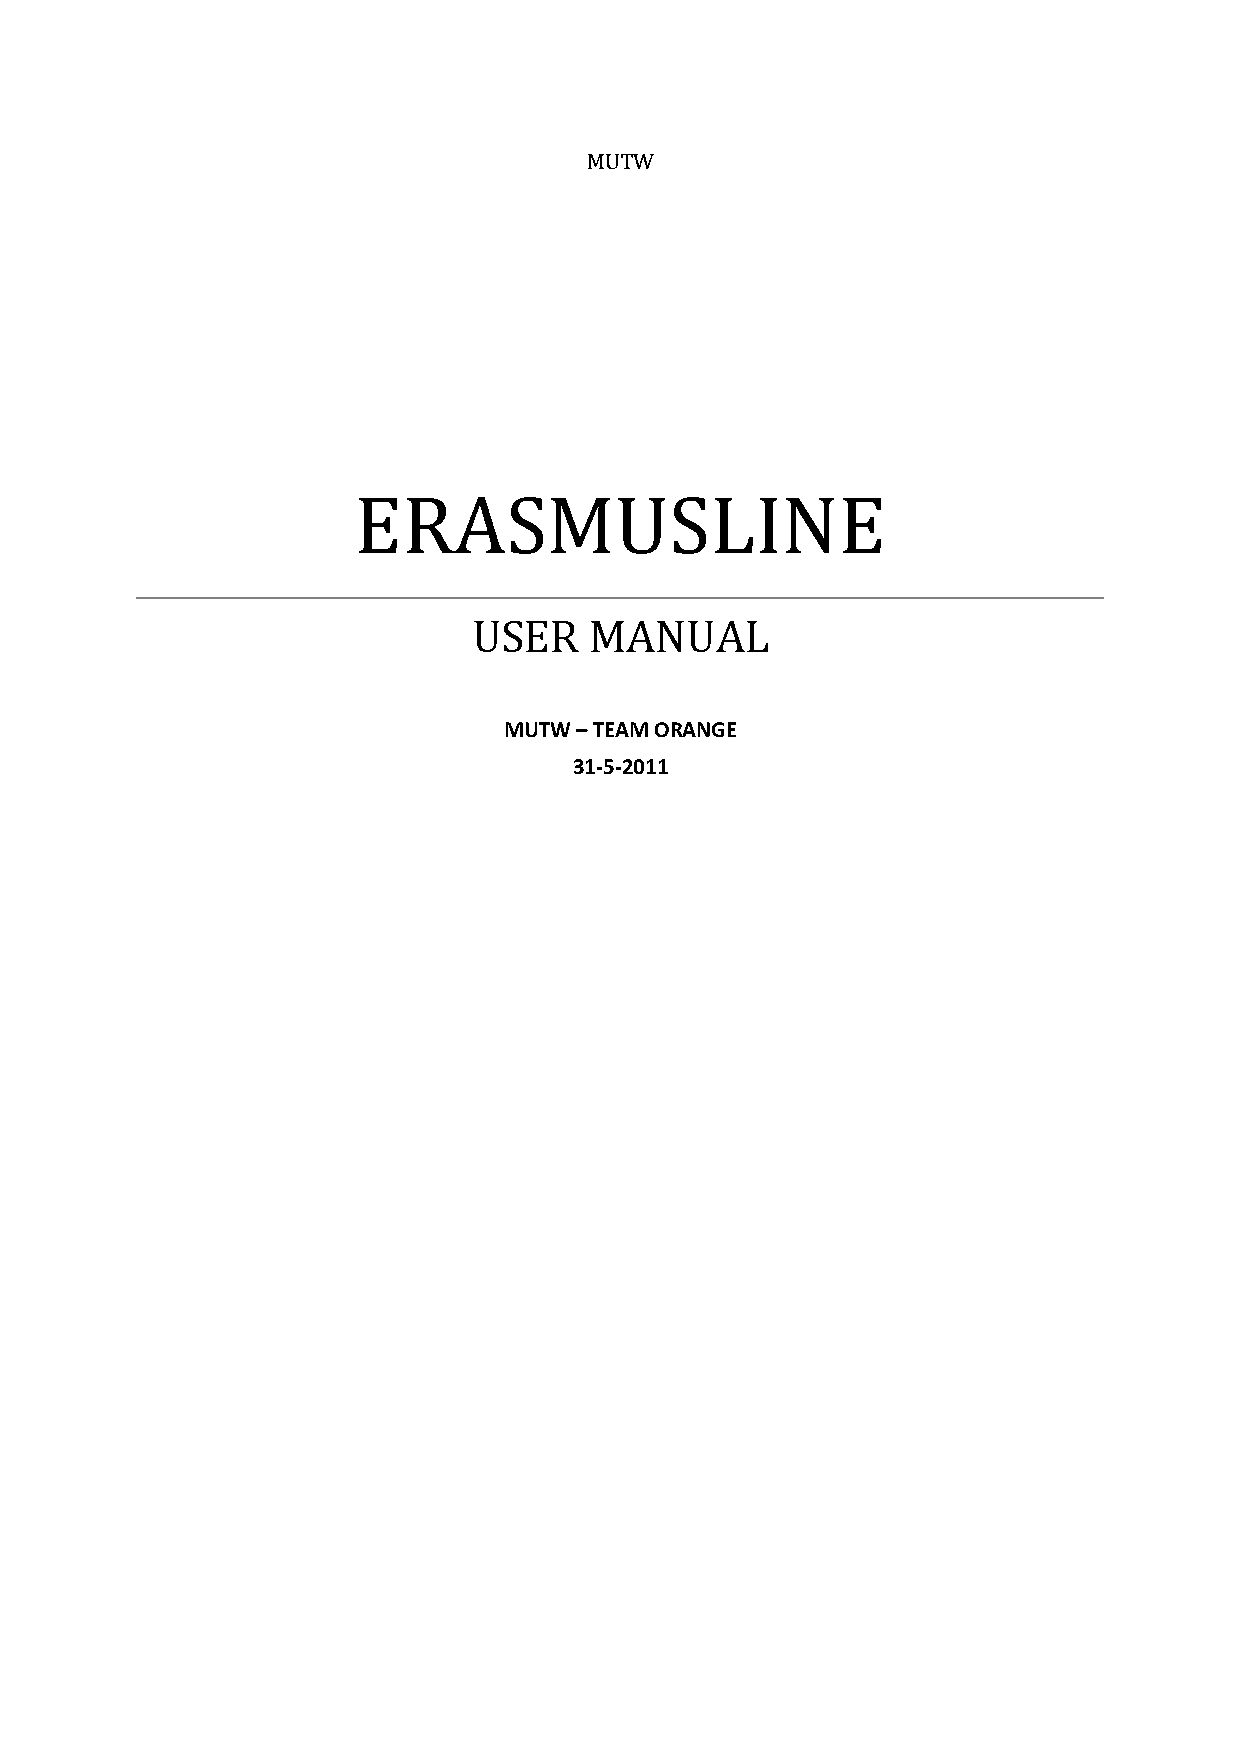
\includepdf{pdf/usermanual.pdf}

\chapter{Appendix 4: EIS Installation and User Manual}
The document in the next page is the available documentation of the Erasmusline
EIS Installation and User Manual, written by the \textbf{P8-STATS} team.

\includepdf{pdf/eis_manual.pdf}
\chapter{Appendix 5: Gantt Chart} \label{apx5}
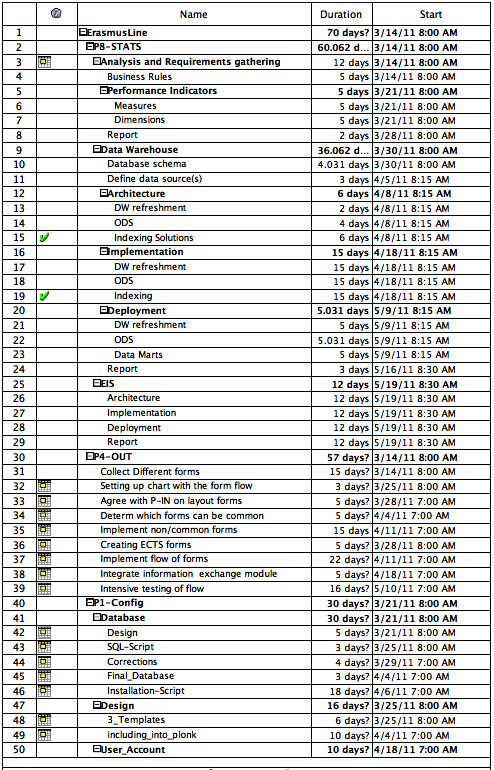
\includegraphics[width=500px,height=560px]{img/gantt1.png} \newpage
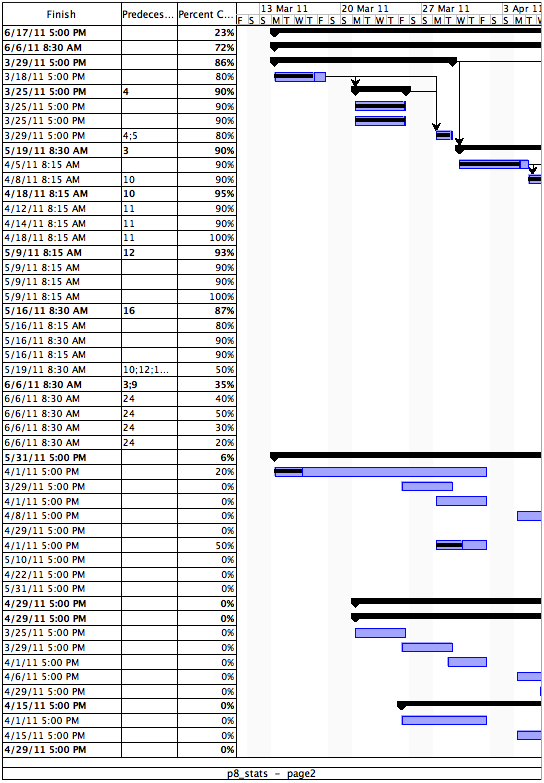
\includegraphics[scale=0.9]{img/gantt2.png} \newpage
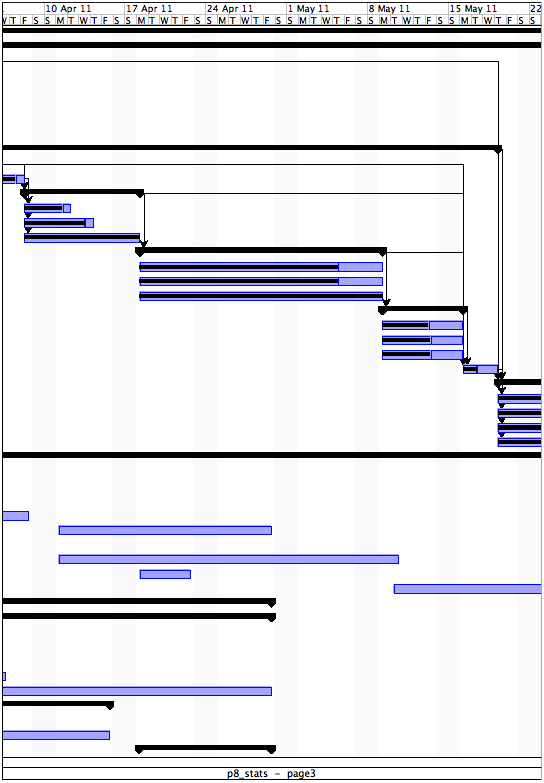
\includegraphics[scale=0.9]{img/gantt3.png} \newpage
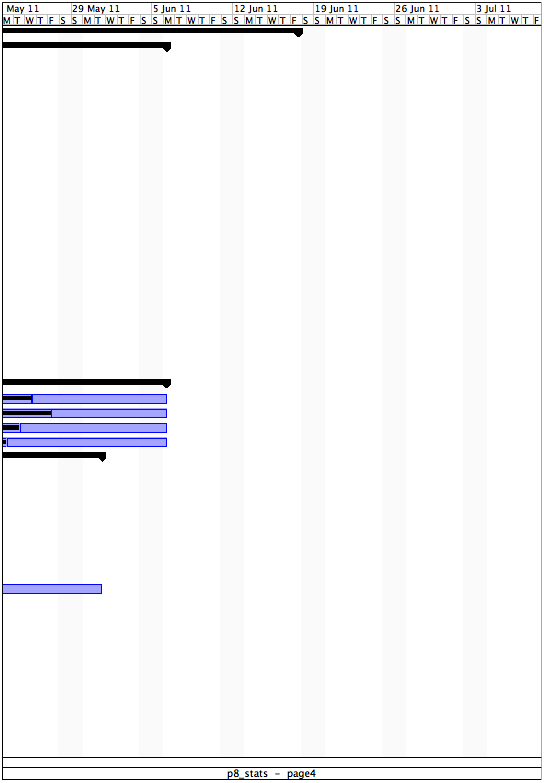
\includegraphics[scale=0.9]{img/gantt4.png} \newpage
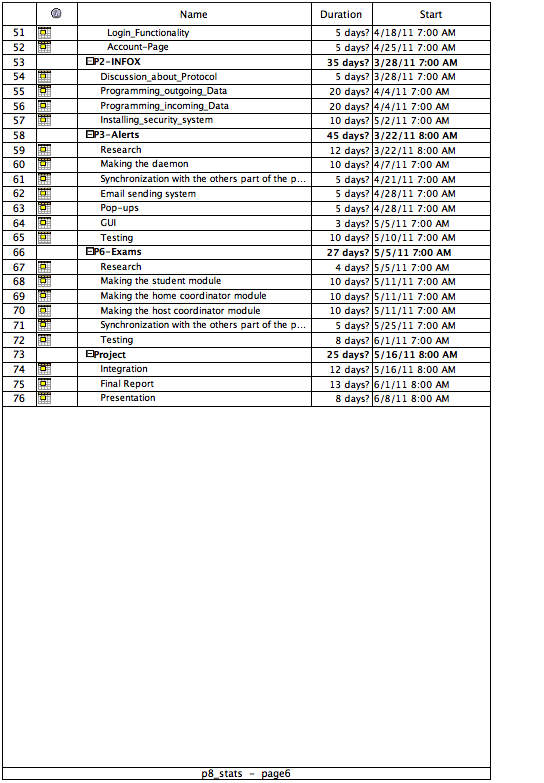
\includegraphics[scale=0.9]{img/gantt5.png} \newpage
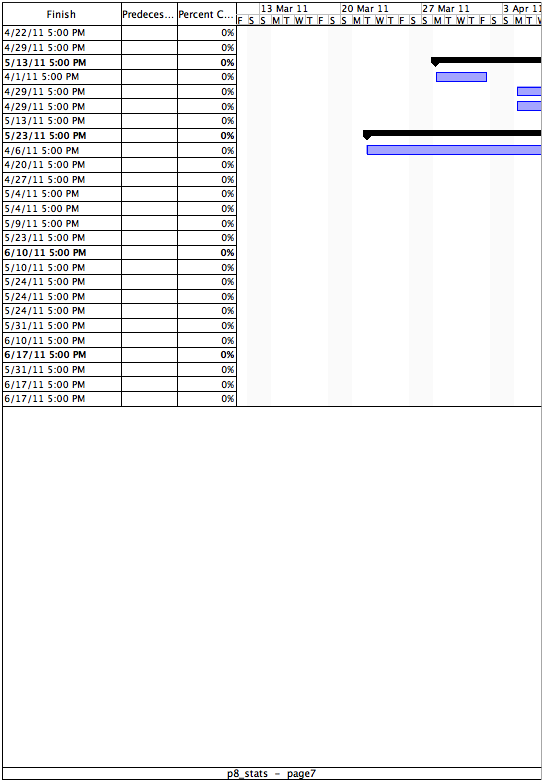
\includegraphics[scale=0.9]{img/gantt6.png} \newpage
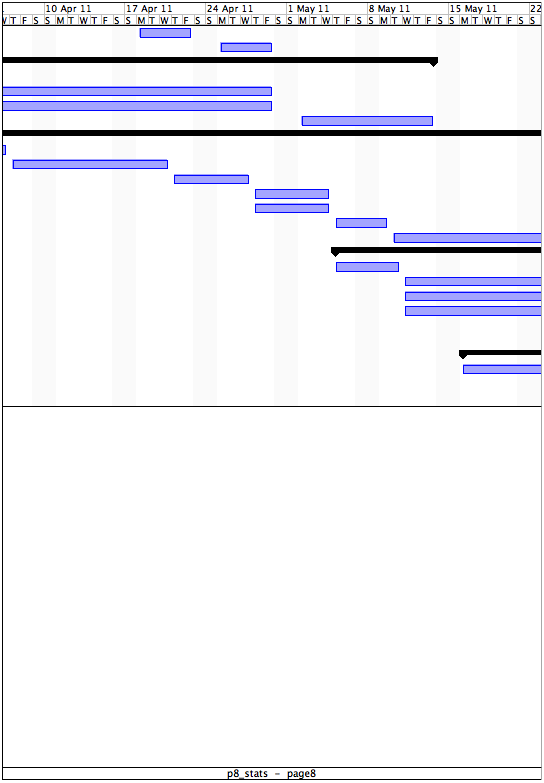
\includegraphics[scale=0.9]{img/gantt7.png} \newpage
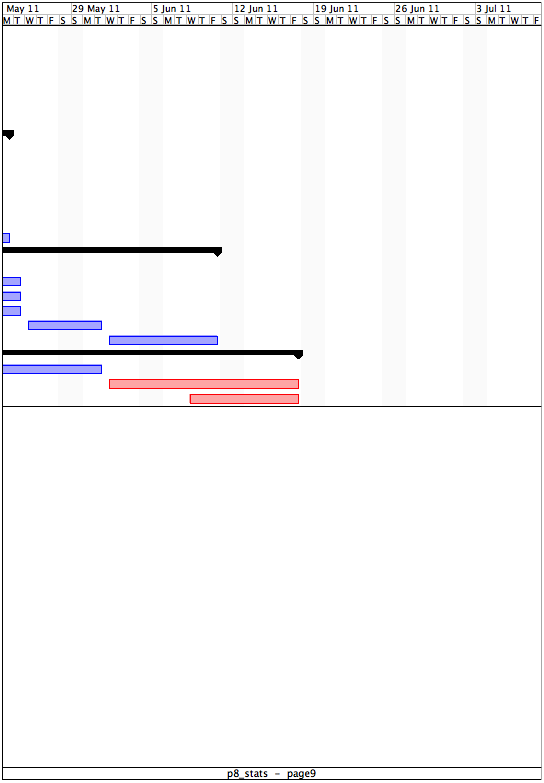
\includegraphics[scale=0.9]{img/gantt8.png} \newpage
\chapter{Appendix 6: Course Matching}
The document in the next page is the available documentation about the course
matching mechanism developed by the \textbf{P7-MATCH} team.
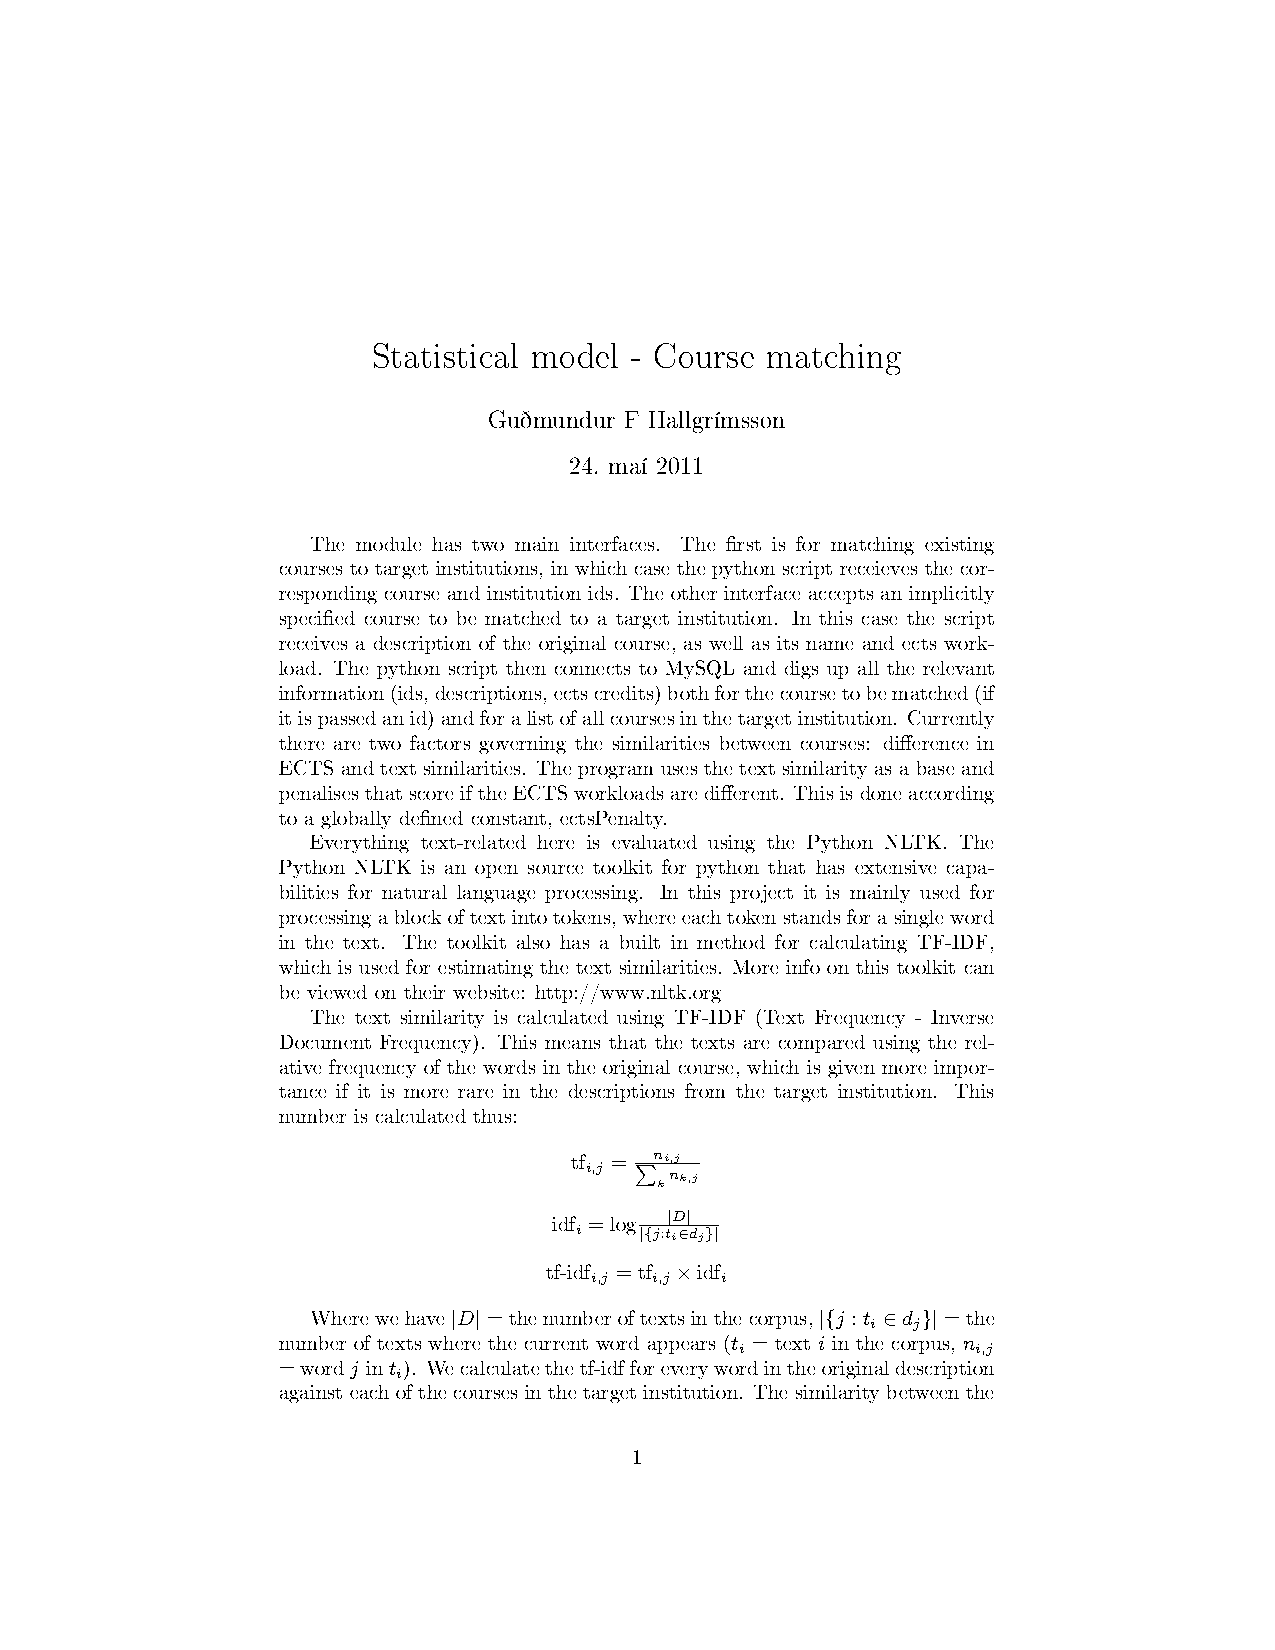
\includepdf{pdf/course_matching.pdf}
\chapter{Appendix 7: The Erasmus Programme - A Statistical Overview}
The document in the next page is the statistical report used to analyse the
amount and scale of real world data and served as guideline in the development
of the P8STATS package.

\includepdf{pdf/statistical_report0809.pdf}

%\addcontentsline{toc}{chapter}{Index}
%\printindex
\end{document} 
